%Standard Dokumenten Einstellungen
%Einstellen der Schriftgröße
\documentclass[a4paper,12pt]{scrreport}

%Einstellen des Seitenabstand
\usepackage[left= 2.5cm,right = 2.5cm, bottom = 4 cm, top = 2.5cm]{geometry}
%zum Ändern des Zeilenabstandes (singlespacing, onehalfspacing, doublespacing), mehr auf https://www.namsu.de/Extra/pakete/Setspace.html
\usepackage[onehalfspacing]{setspace}

%Schriftart
\usepackage[T1]{fontenc}
%Schriftarten Paket in die {} einfügen
\usepackage{}

%Fußzeile
\usepackage[headsepline=1pt, footsepline=1pt]{scrlayer-scrpage}
\renewcommand*\chapterpagestyle{scrheadings}
\pagestyle{scrheadings}
\ihead{\Vorname{} \Nachname{}}
\ohead{\Art{}}


%===============================================================================
% Standard Packages

%Für das einfügen von Bildern
\usepackage{graphicx}
%Pfad zu den Bildern --> Bei Verwendung eines Bildes in includegraphics muss nur der Name des Bildes genannt werden, z.B. DHBW_Logo
\graphicspath{{Pictures/}}
\usepackage{subcaption}

%Für weitere komplexere Grafiken und Positionierung, mehr auf https://www.overleaf.com/learn/latex/TikZ_package
\usepackage{tikz}

%Für schönere Tabellen, mehr auf https://www.namsu.de/Extra/pakete/Tabularx.html
\usepackage{tabularx}
%Zum einfügen von PDF Dateien, mehr auf https://www.namsu.de/Extra/pakete/Pdfpages.html
\usepackage{pdfpages}

%Für das Literaturverzeichnis, ändern von style, ändert die Art der Zitierung und des Verzeichnis, mehr auf https://www.overleaf.com/learn/latex/Biblatex_bibliography_styles
\usepackage[style = authortitle]{biblatex}
\bibliography{Directorys/Literatur}{}

%Fügt Abkürzungsverzeichnis hinzu
%Hinzufügen von "printonlyused" in eckige Klammern, um nur verwendete Abkürzungen darzustellen
\usepackage[]{acronym}

% zusätzliche Schriftzeichen der American Mathematical Society
\usepackage{amsfonts}
\usepackage{amsmath}

%Pakete für die Deutsche Sprache
\usepackage[ngerman]{babel}
\usepackage{csquotes}

%Für Code
\usepackage{float}
\usepackage{fancyvrb}

%Für Links und Hyperlinks
\usepackage[colorlinks = true,
            linkcolor = black,
            urlcolor  = blue,
            citecolor = black]{hyperref}

%===============================================================================
%Felder Ausfüllen, sie geben den Inhalt des Titelblatt an
%Inhalt der Titelseite
\newcommand{\Titel}{Titel der Projektarbeit}
\newcommand{\Art}{Projektarbeit}
\newcommand{\Vorname}{Max}
\newcommand{\Nachname}{Mustermann}
\newcommand{\Studiengang}{Studiengang}
\newcommand{\Abgabedatum}{01.01.1111}
\newcommand{\Bearbeitungszeitraum}{12 Wochen}
\newcommand{\Matrikelnummer}{9999999999}
\newcommand{\Kurskrzl}{Kurzkürzel}
\newcommand{\Ausbildungsfirma}{Firma}
%Benötigt bei Elektrotechnik Titelseite
\newcommand{\Abteilung}{Abteilung}
\newcommand{\Standort}{Standort}
\newcommand{\BetreuerFirma}{Titel Vorname Nachname}
\newcommand{\BetreuerDHBW}{Titel Vorname Nachname}

%Nur benötigt wenn Sperrvermerk verwendet wird
\newcommand{\SperrvermerkAuslaufDatum}{31.12.2222}


%===============================================================================
%Start des Dokuments
\begin{document}

%Die Gliederung entspricht den Richtlinien der Informationstechnik Fakultät, bitte anpassen für die jeweiligen Richtlinien

%Titelblatt
\pagestyle{empty}
% Wichtig, damit man nicht immer von Vorlage.tex bauen muss
% !TEX root = ../Vorlage.tex

%===========Logos============================================
%DHBW_Logo
\begin{tikzpicture}[remember picture,overlay]
 \node[anchor=north east,inner xsep=50pt, inner ysep=25pt] at (current page.north east)
 {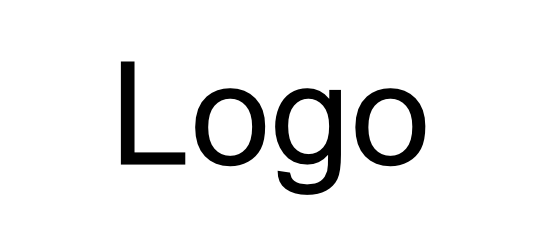
\includegraphics[scale=0.25]{DHBW_Logo}};
\end{tikzpicture}

%Firmen Logo
\begin{tikzpicture}[remember picture,overlay]
   \node[anchor=north west,inner xsep=50pt, inner ysep=25pt] at (current page.north west)
              {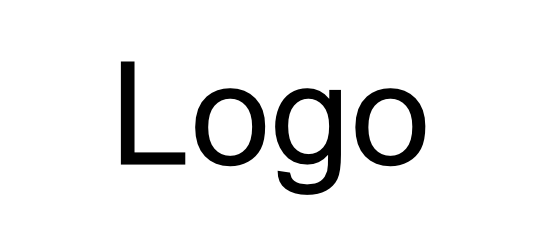
\includegraphics[scale=0.2]{ABB_Logo}};
\end{tikzpicture}

%===========Inhalt===========================================
\vspace{1cm}

\begin{center}
 \large{\Titel}
\end{center}

\vspace{1cm}

\begin{center}
 \textbf{\Art}
\end{center}

\vspace{4cm}

\begin{center}
 des Studienganges \Studiengang \\
 an der Dualen Hochschule Baden-Württemberg Mannheim
\end{center}

\vspace{0.75cm}

\begin{center}
 von\\
 \Vorname{} \Nachname
\end{center}

\vspace{1cm}

\begin{center}
 \Abgabedatum
\end{center}

\vspace{2cm}

\begin{tabular}{l@{\hspace{2cm}}l}
 Bearbeitungszeitraum:            & \Bearbeitungszeitraum        \\
 Matrikelnummer, Kurs:            & \Matrikelnummer, \Kurskrzl   \\
 Ausbildungsfirma:                & \Ausbildungsfirma, \Standort \\
 Betreuer der Ausbildungsfirma:   & \BetreuerFirma               \\
 %Gutachter der Dualen Hochschule: & \BetreuerDHBW                \\
                                                                 \\
                                                                 \\
\cline{2-2} & Unterschrift (Betreuer)
\end{tabular}

%% Wichtig, damit man nicht immer von Vorlage.tex bauen muss
%!TEX root = ../Vorlage.tex

%===========Logos============================================
%DHBW_Logo
\begin{tikzpicture}[remember picture,overlay]
 \node[anchor=north east,inner xsep=50pt, inner ysep=25pt] at (current page.north east)
 {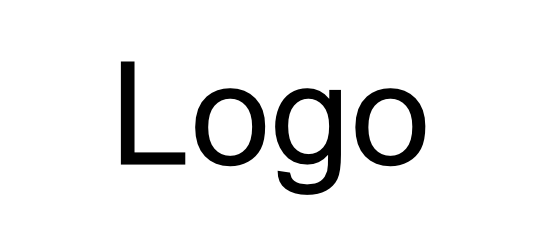
\includegraphics[scale=0.25]{DHBW_Logo}};
\end{tikzpicture}

%Firmen Logo
\begin{tikzpicture}[remember picture,overlay]
 \node[anchor=north west,inner xsep=50pt, inner ysep=25pt] at (current page.north west)
 {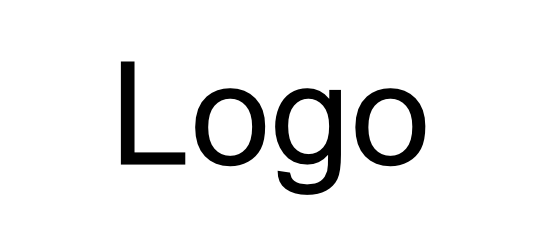
\includegraphics[scale=0.2]{ABB_Logo}};
\end{tikzpicture}

%===========Inhalt===========================================
\vspace{0.5cm}

\begin{center}
 \large{\Titel}
\end{center}

\vspace{0.5cm}

\begin{center}
 \textbf{\Art}
\end{center}

\vspace{2.5cm}

\begin{center}
 des Studienganges \Studiengang \\
 an der Dualen Hochschule Baden-Württemberg Mannheim
\end{center}

\vspace{0.5cm}

\begin{center}
 von\\
 \Vorname{} \Nachname
\end{center}

\vspace{0.5cm}

\begin{center}
 \Abgabedatum
\end{center}

\vspace{0.5cm}

\begin{tabular}{l@{\hspace{2cm}}l}
 Bearbeitungszeitraum:            & \Bearbeitungszeitraum        \\
 Matrikelnummer, Kurs:            & \Matrikelnummer, \Kurskrzl   \\
 Ausbildungsfirma, Abteilung:     & \Ausbildungsfirma, \Abteilung\\
 Standort:                        & \Standort                    \\
 Betreuer der Ausbildungsfirma:   & \BetreuerFirma               \\\\\\\cline{2-2}
 %Gutachter der Dualen Hochschule: & \BetreuerDHBW
                                  & Unterschrift (Betreuer)
\end{tabular}


%Sperrvermerk
\pagestyle{empty}
% !TEX root = ../Vorlage.tex
\chapter*{Sperrvermerk}
\glqq Der Inhalt dieser Arbeit darf weder als Ganzes noch in Auszügen Personen außerhalb des Prüfungsprozesses und des Evaluationsverfahrens zugänglich gemacht werden, sofern keine anders
lautende Genehmigung des Dualen Partners vorliegt.\grqq{} [Ende der Sperrfrist: \SperrvermerkAuslaufDatum]

%% !TEX root = ../Vorlage.tex
\chapter*{Sperrvermerk}
\addcontentsline{toc}{chapter}{Sperrvermerk}
Dieser Bericht enthält vertrauliche Daten der ABB Automation GmbH in Mannheim. Jegliche Vervielfältigung oder Veröffentlichung von Inhalten, Resultaten oder Zusammenfassungen ist nur mit ausdrücklicher schriftlicher Genehmigung der ABB Automation GmbH und unter Benachrichtigung des Autors gestattet.

\vspace{1.5cm}

\begin{tabularx}{0.9\textwidth}[b]{p{7cm} X p{7cm}}
\cline{1-1} \cline{3-3}
Ort, Datum &  & Unterschrift(Betreuer)
\end{tabularx}

%Der Inhalt dieser Arbeit darf weder als Ganzes noch in Auszügen Personen außerhalb des Prüfungsprozesses und des Evaluationsverfahrens zugänglich gemacht werden, sofern keine anders lautende Genehmigung des Dualen Partners vorliegt.
%[Ende der Sperrfrist: \SperrvermerkAuslaufDatum]


\pagenumbering{Roman}

%Eigenleistung
% Wichtig, damit man nicht immer von Vorlage.tex bauen muss
% !TEX root = ../Vorlage.tex
\chapter*{Erklärung}

Ich versichere hiermit, dass ich meine Bachelorarbeit (bzw. Studien- und Projektarbeit) mit dem
Thema: \Titel selbstständig verfasst und keine anderen als die angegebenen Quellen und Hilfsmittel
benutzt habe.
Ich versichere zudem, dass die eingereichte elektronische Fassung mit der gedruckten Fassung
übereinstimmt. *\\
\small{* falls beide Fassungen gefordert sind}\\[3cm]
\begin{tabularx}{\textwidth}[b]{p{5cm} X p{5cm}} \cline{1-1} \cline{3-3}
 Ort, Datum &  & Unterschrift 
\end{tabularx}


%Abstract
%% !TEX root = ../Vorlage.tex
\chapter*{Abstract}
Hier kommt dein Abstract rein.

% !TEX root = ../Vorlage.tex
\chapter*{Abstract}
Hier kommt dein Abstract rein.


%Tabelle Überblick Tätigkeiten (Elektrotechnik)
\include{Sections-Default/Ueberblick_Taetigkeiten}

%===================================================
%Verzeichnisse: Verwendete Verzeichnisse Aktivieren durch entfernen von: % vor dem \
%Inhaltsverzeichnis
%\addcontentsline{toc}{chapter}{Inhaltsverzeichnis}\tableofcontents\clearpage

%Abbildungsverzeichnis
%\addcontentsline{toc}{chapter}{Abbildungsverzeichnis}\listoffigures\clearpage

%Tabellenverzeichnis
%\addcontentsline{toc}{chapter}{Tabellenverzeichnis}\listoftables\clearpage

%Abkürzungsverzeichnis
%\include{Directorys/Abkürzungsverzeichnis}
%===============================================================================

%Vorwort: Um Vorwort zu verwenden, % entfernen
%% !TEX root = ../Vorlage.tex
\chapter*{Vorwort}
Hier kannst du dein Vorwort hinschreiben.


\pagestyle{scrheadings}
\pagenumbering{arabic}
%===============================================================================

%Eigene Kapitel
%Kapitel als eigene .tex datei erstellen und einbinden mit: \include{Pfad/Dateiname}
% !TeX root = ../template.tex

\chapter{Beispiel Kapitel}
Die Datei zu diesem Kapitel findest du im Sections Ordner, als Example.tex.\\
In dieser Datei geht es darum euch einen Einblick in die Verwendung der Kommandos aus der Dokumentation Kapitel 3 zu geben \footcite{doku}.
\section{Aufzählungen}
Dort wird gezeigt wie man eine Aufzählung macht:
\begin{itemize}
 \item Erster Stichpunkt
 \item Zweiter Stichpunkt
\end{itemize}
Oder auch wie diese Nummeriert dargestellt werden können.
\begin{enumerate}
 \item Erster Stichpunkt
 \item Zweiter Stichpunkt
\end{enumerate}
\section{Bilder}
Zudem wird gezeigt wie man Bilder einfügt und diese referenzieren kann.
\begin{center}
 \begin{figure}[h!]
  \centering
  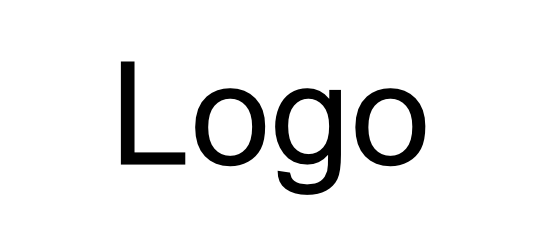
\includegraphics[scale = 0.3]{dhbw-logo}
  \caption{Dies ist ein Logo, link zu DHBW Logo ist in Pictures/downloads.txt zu finden}
  \label{fig:dhbwlogo}
 \end{figure}
\end{center}
Sowie zum Beispiel \ref{fig:dhbwlogo} referenziert wird.
\section{Zitieren}
Ein weiterer Teil ist, wie zitiert wird, ob auf \glqq{}Deutsche\grqq{} oder auf ``Englische'' Art und Weise\footcite[3.2]{doku}.


%===============================================================================
\pagenumbering{Roman}
%Literaturverzeichnis
\addcontentsline{toc}{chapter}{Literaturverzeichnis}\printbibliography[title=Literaturverzeichnis]
%Anhang

\end{document}
